\subsection{Approval, Execution, and Evidence}
\label{sec:mech}

\begin{figure}[t]
\centering
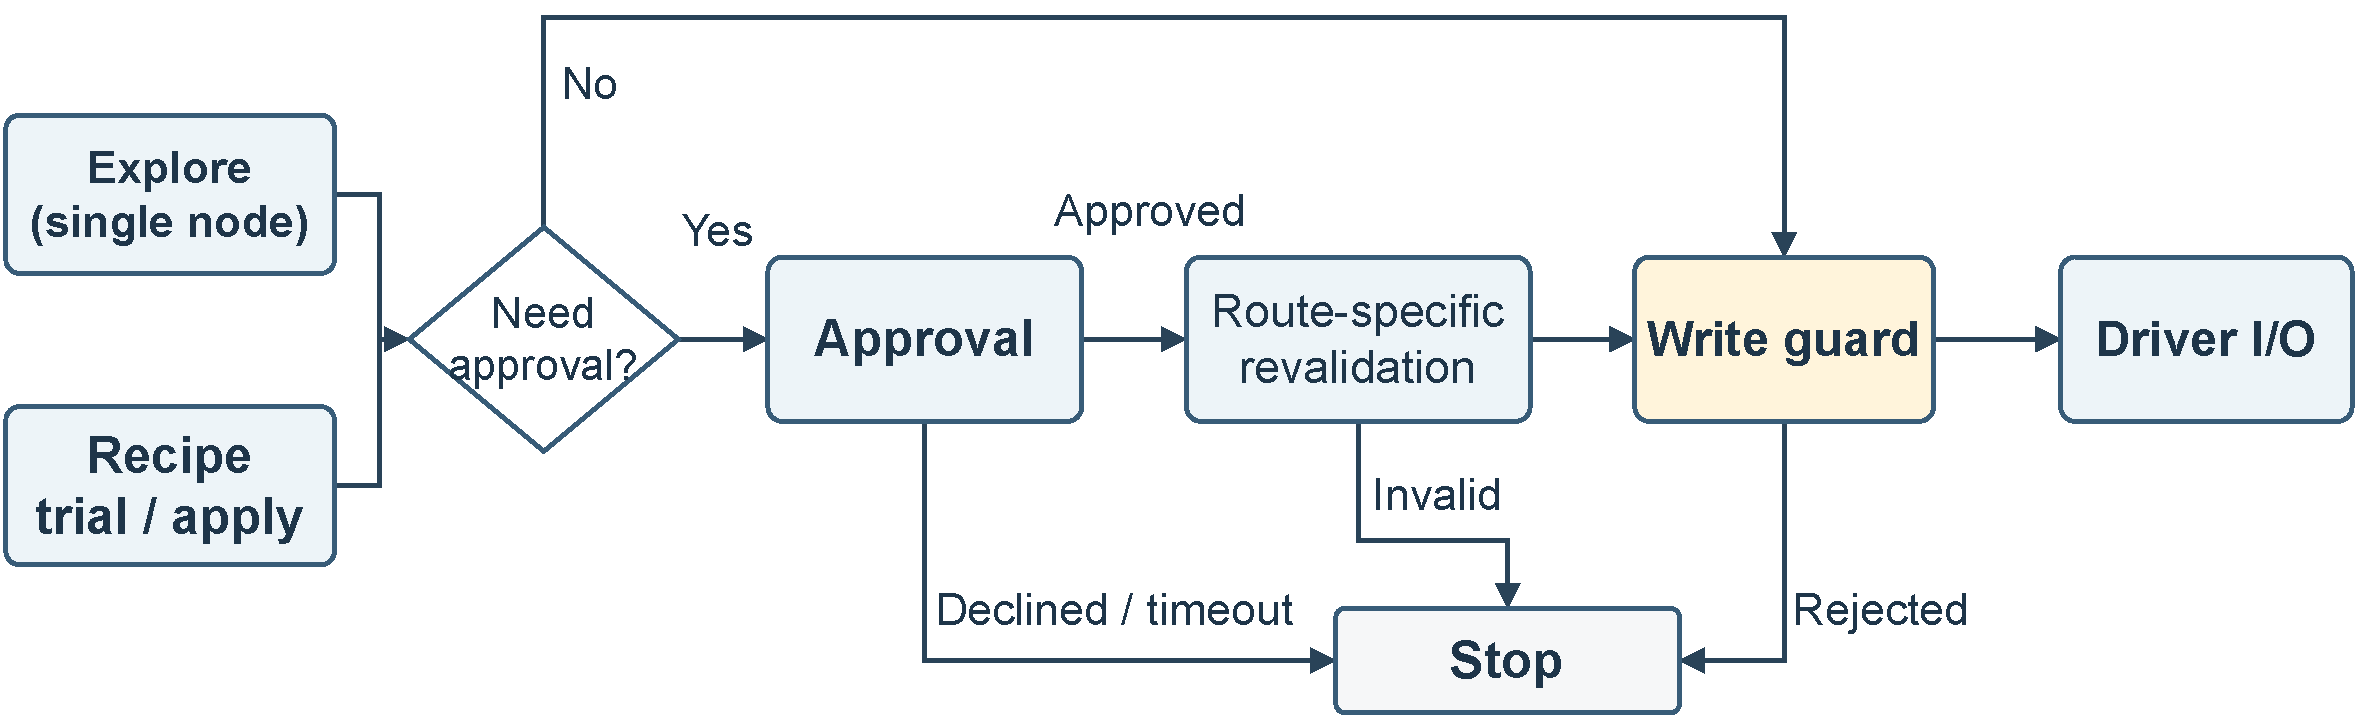
\includegraphics[width=\columnwidth]{resources/fig4-governed-flow.pdf}
\caption{Route map of the governed write paths, complementing the single-node sequence in Algorithm~1. Single-node \texttt{optimization\_explore} intents and recipe trial or apply operations take route-specific approval and revalidation before converging on the shared write guard of Eq.~(\ref{eq:admission}). A decline, timeout, failed revalidation, or guard rejection stops the affected operation or parameter before driver dispatch; command outcomes, setpoint readbacks, and later observations remain distinct records. Other applicable dispatch and authorization checks are omitted; bypassing approval does not bypass them.}
\label{fig:hitl}
\end{figure}
Fig.~\ref{fig:hitl} maps both write routes onto the shared write guard and the distinct records returned after dispatch; Algorithm~1 details the single-node check sequence. For a manual single-node \texttt{optimization\_explore} request, approval covers the node, proposed value, current effective interval, and rationale. The same boundary receives an agent's typed intent after acquisition and analysis. As in Algorithm~1, a decline or timeout stops the request. Approval triggers revalidation of the original direct node binding or, for a recipe operation, the recipe binding and parameter membership. Single-node approval does not use the recipe-operation context snapshot described next. In either path, revalidation does not make the checks and external device write atomic.

Recipe operations use a separate approval path. For \texttt{recipe\_trial} and \texttt{recipe\_apply}, approval is bound to the recipe operation and
active line--product--recipe--run context. After approval, the handler checks
authority and context again and verifies the recipe definition and
candidate scope before dispatch. A changed context, revoked binding, or
changed recipe definition prevents that proposal from proceeding. Recipe
trial approvals default to a 30-minute window; single-node approval waits
expire after 180\,s. Outside benchmark mode, agent and manual
writes are subject to a minimum 60-s interval following a setpoint change;
recipe trials also use a per-line cadence of 300\,s by default.

A \texttt{recipe\_trial} submits a bounded batch from the agent's control intent through the configured
driver and returns a result for each parameter to the calling route. Parameters are attempted
individually, so a batch can be partially applied; results and device state must be reconciled before any retry. A trial does not save or apply a recipe
version, and before updating, applying, or rolling back the recipe, the caller can retrieve later DAQ observations separately.

As sketched in Fig.~\ref{fig:hitl}, receipts record the command outcome returned to the agent or caller; observations record what followed in
the process. Command results are graded as readback-verified,
transport-acknowledged, or unverified. When a successful recipe write is not
already readback-verified, the service may, by default, attempt up to three additional
reads at 2\,s intervals where supported; recipe batches retain verification
outcomes for each parameter. A readback-verified result means that the
returned value matched the request within the applicable tolerance. A transport
acknowledgment alone does not establish that the device applied the value, and
an unverified result does not establish a matching readback. DAQ stores later
timestamped process observations for the agent's next analysis turn, while
recipe history, approvals, and task records remain with their owning services.
Identifiers and timestamps can link these records when available, but a later
observation alone does not prove that the command caused the measured change.

